\section{Gaussian Mixture Model}

Gaussian mixture models make the assumption that data is generated from Gaussians. To be more precise a convex-combination of Gaussian distributions:
$$p(x \; | \; \theta) = p(x \; | \; \mu, \Sigma, w) = \sum_{j=1}^k w_j \cdot \mathcal{N}(x; \mu_j, \Sigma_j)$$

\begin{center}
	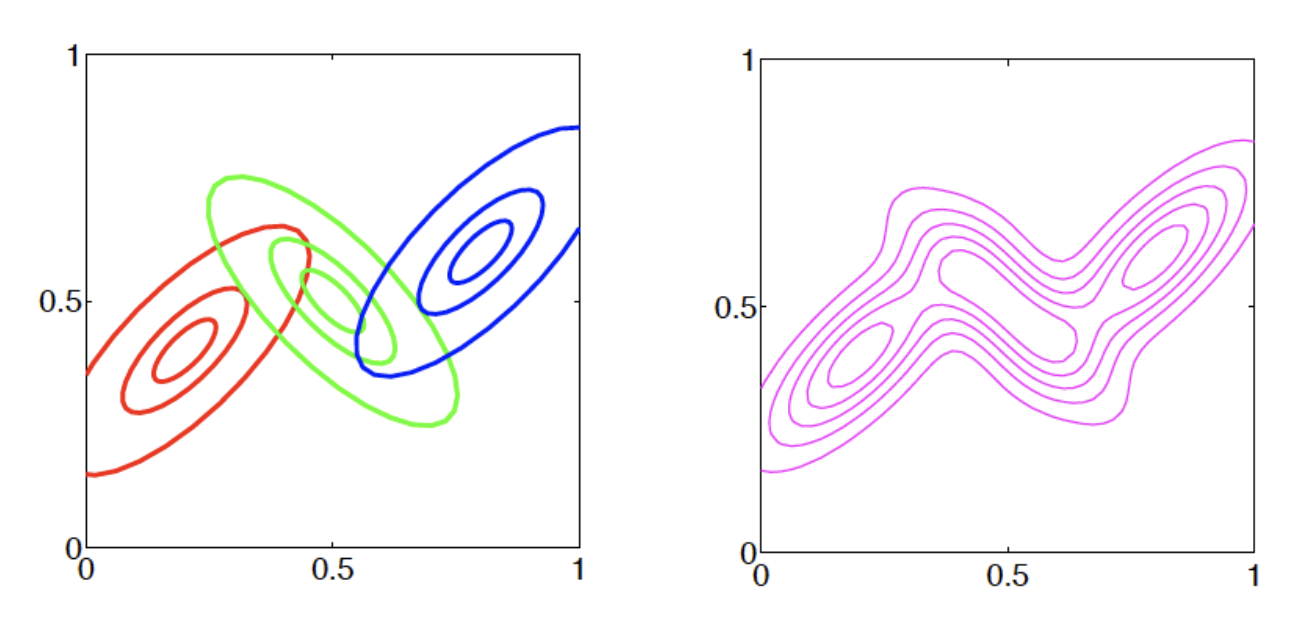
\includegraphics[width=\columnwidth]{gmm.png}
\end{center}

We do not know the labels $z$ for the data and can only see the level-set on the right, now we want to cluster this data. The problem we try to solve is to estimate the parameters for the Gaussian distributions (minimize log-likelihood).
$$(w_{i:k}^*, \mu_{i:k}^*, \Sigma_{1:k}^*) = \argmin \; - \sum_{i=1}^n \log \sum_{j=1}^k w_j \cdot \mathcal{N}(x_i \; | \; \mu_j, \Sigma_j)$$

This is a non-convex objective, but we can still try to apply SGD. But there is a better way to fit this model. The idea is that fitting a GMM is similar to training a GBC without labels. We want to apply an iterative approach where we first start with some guess for our parameters, predict the unknown labels and then impute the missing data. Now we can get a closed form update for our model which we then use to refine our parameters.

\subsection{Hard-EM Algorithm}

First we are gonna look at the simpler version of the EM (expectation maximization) algorithm:
\begin{itemize}
	\item Initialize the parameters $\theta^{(0)}$
	\item For $t = 1,2,...$ :
		\begin{itemize}
			\item \textbf{E-Step}: predict the most likely class for each data point:
				\begin{align*}
					z_i^{(t)} &= \argmax{z} \; p(z \; | \; x_i, \theta^{(t-1)}) \\
					&= \argmax{z} \; p(z \; | \; \theta^{(t-1)}) \cdot p(x_i \; | \; z, \theta^{(t-1)}))
				\end{align*}
			\item \textbf{M-Step}: compute MLE of $\theta^{(0)}$ as for GBC
		\end{itemize}
\end{itemize}

There are some problems with this approach, for one points are assigned a label even though the model is uncertain. Further it tries to extract too much information from a single point. In practice, this may work poorly if clusters are overlapping. Hard-EM with uniform weights and spherical covariances is equivalent to k-Means with Lloyd's heuristics.

\subsection{Soft-EM Algorithm}

Instead of predicting hard class assignments for each data point we want to predict class probabilities. 
\begin{itemize}
	\item Initialize the parameters $\theta^{(0)}$
	\item For $t = 1,2,...$ :
		\begin{itemize}
			\item \textbf{E-Step}: calculate the cluster membership weights for each point:
				\begin{align*}
					\gamma_j^{(t)}(x_i) &= p(z_i = j \; | \; x_i, \theta_j^{(t-1)}) \\
					&= \frac{w_j \cdot p(x_i ; \theta_j^{(t-1)})}{\sum_k w_k \cdot p(x_i ; \theta_k^{(t-1)})}
				\end{align*}
			\item \textbf{M-Step}: compute MLE with closed form solution:
				\begin{align*}
			 		w_j^{(t)} &= \frac{1}{n} \sum_{i=1}^n \gamma_j^{(t)}(x_i) \quad \; \mu_j^{(t)} = \frac{\sum_{i=1}^n x_i \cdot \gamma_j^{(t)}(x_i)}{\sum_{i=1}^n \gamma_j^{(t)}(x_i)} \\
			 		\Sigma_j^{(t)} &= \frac{\sum_{i=1}^n \gamma_j^{(t)}(x_i)(x_i - \mu_j^{(t)})(x_i - \mu_j^{(t)})^\top}{\sum_{i=1}^n \gamma_j^{(t)}(x_i)}
			 	\end{align*}
		\end{itemize}
\end{itemize}à

In general, Soft-EM will typically result in higher likelihood values, as it can better deal with "overlapping" clusters. When speaking of EM we usually refer to Soft-EM. \smallskip

The EM algorithm is sensitive to initialization. We usually initialize the weights as uniformly distributed, the means randomly or with k-Means++ and for variances we use spherical initialization or empirical covariance of the data. To select $k$, in contrast to k-Means, we can use cross-validation.

\subsection{Degeneracy of GMMs}

GMMs can overfit when only having limited data, we want to avoid that the Gaussians get too narrow and fit to a single data point. To avoid this we add $v^2 I$ to our variance. This makes sure that the variance does not collapse and is equivalent to placing a Wishart prior the covariance matrix, and computing the MAP. We choose $v$ by cross-validation.

\subsection{Gaussian-Mixture Bayes Classifiers}

We can also use GMMs for classification tasks, by assuming that the conditional distribution for each class can be modelled by a GMM.

$$p(x \; | \; y) = \sum_{j=1}^{k_y} w_j^{(y)} \mathcal{N}(x; \mu_j^{(y)}, \Sigma_j^{(y)})$$

We can then use this model for classification, giving us highly complex decision boundaries:

$$p(y \; | \; x) = \frac{1}{z} p(y)  \sum_{j=1}^{k_y} w_j^{(y)} \mathcal{N}(x; \mu_j^{(y)}, \Sigma_j^{(y)})$$

\begin{center}
	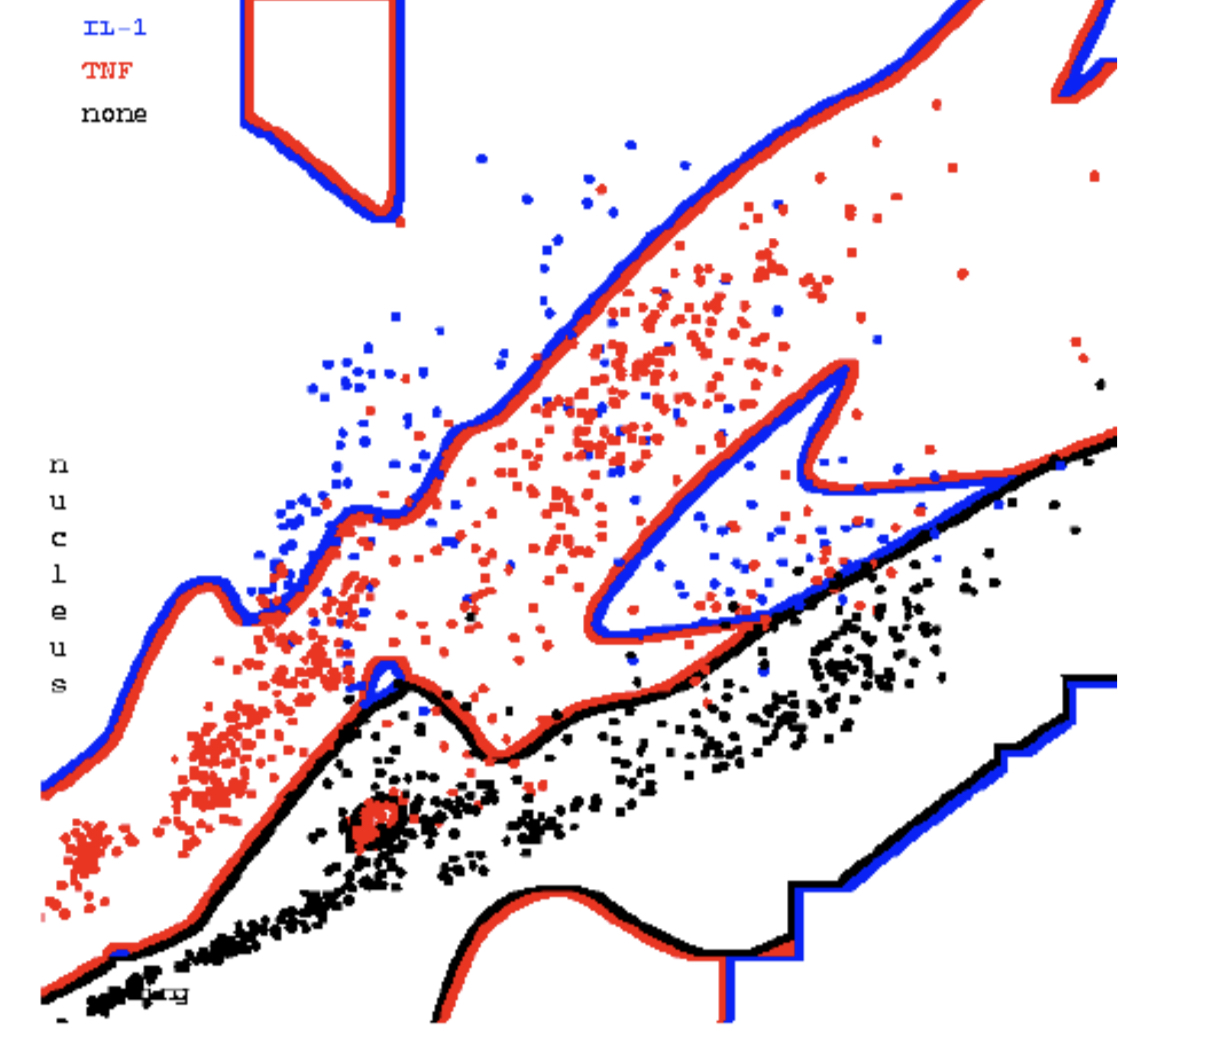
\includegraphics[width=0.7\columnwidth]{gmmb.jpeg}
\end{center}

\subsection{GMMs for Density Estimation}

So far, we used GMMs primarily for clustering and classification. Another natural use case for GMMs is density estimation, which in turn can be used for anomaly detection or data imputation.

\begin{center}
	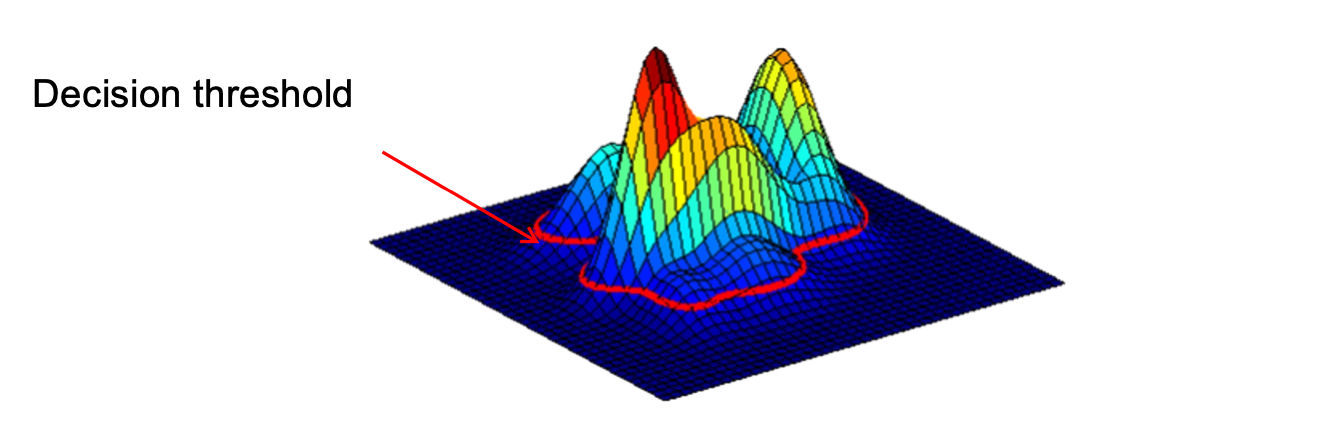
\includegraphics[width=\columnwidth]{anomaly-detection-gmm.png}
\end{center}

To determine outliers, we simply compare the estimated density of a data point against a threshold value $\tau$. This allows us to control the FP rate. As we vary the threshold we trade FPs and FNs. We can use ROC curves as evaluation criterion and optimize using cross-validation to find the optimal value for $\tau$.

\subsection{General EM Algorithm}

The framework of soft EM can also be used for more general distributions than gaussians. We formulate the two steps:
\begin{itemize}
	\item \textbf{E-Step}: Take the \textbf{expected} value over latent variables to generate a likelihood function $Q(\theta ; \theta^{(t-1)})$:
		\begin{align*}
			Q(\theta ; \theta^{(t-1)}) &= \E_{Z}[ \log  p(X, Z \; | \; \theta) \; | \; X, \theta^{(t-1)}] \\
			&= \sum_{i=1}^n \sum_{z_i=1}^k \gamma_{z_i}(x_i) \log p(x_i, z_i \; | \; \theta)
		\end{align*}
		with $\gamma_z(x) = p(z \; | \; x, \theta^{(t-1)})$
	\item \textbf{M-Step}: Compute MLE / \textbf{Maximize}:
		$$\theta^{(t)} = \argmax{\theta} \; Q(\theta; \theta^{(t-1)})$$
\end{itemize}

It is important to note that we have guaranteed mono- tonic convergence, where each EM-iteration monotonically increases the data likelihood.
